\section{Example of a 2-Way Join}
Correlating features across separate datasets requires first joining these datasets. Correlation coefficients ($r$) between different admissions benchmarking methods and CSC1015F course results are calculated according to the inner join shown in Equation \ref{eq:2-way-join}. A single student number may appear multiple times in the grades data if a student repeated a course, but should appear only once on the admissions data, for the first time they registered at UCT. Rows for student numbers found in the admissions data but not the grades data are not used, nor are rows found for students in the grades data but not the admissions data.

\subsection{ETL}
Using nETL, rows are extracted from the two CSV files (\textit{Admissions (2014 - 2016).csv} and \textit{Grades (2014 - 2016).csv}) concurrently and independently of each other, in batches of 5 000 and 10 000 rows respectively.

Through nETL configuration, rows from the admissions data are selected for students who are South African citizens or permanents residents, and who are undergraduates. Rows from the grades data are selected for students who attended CSC1015F during 2014, 2015, or 2016. Since the admissions data doesn't have a field for course year, a natural join with grades on the \textit{anonIDnew} field is performed via nETL ($admissions \bowtie grades$) to retrieve a list of students who attended CSC1015F. Using this list, rows are selected from the admissions data for students who attended CSC1015F.

Rows retrieved from the CSVs contain numerous fields that are not required, and so nETL is configured to apply an attribute-whitelisting process to both admissions and grades data. Batches of objects are serialized to JSON strings and loaded into a single CouchDB database using the \textit{\_bulk\_docs} endpoint. An example of a row from grades data serialized to a JSON string and loaded into CouchDB is shown in Figure \ref{fig-json-grade}.

\begin{figure}[H]
    \centering
    \begin{mdframed}
        \centering
        \begin{minted}{text}
{
    "_id": "7530f4eed7e6bc3ef0d99a53be8ba9a2",
    "_rev": "8-232d0cf39728d41b4c5935f12469209d",
    "RegAcadYear": 2016,
    "anonIDnew": 1,
    "Course": "CSC1015F",
    "Percent": "55",
    "type_": "grade"
}    
        \end{minted}
    \end{mdframed}
    \caption[Serialized grades document]{\textbf{Figure \ref{fig-json-grade}: Serialized grades document}}
    \label{fig-json-grade}
\end{figure}

\subsection{Indexing}
After loading the data from the CSVs into CouchDB, a Map function is used to produce an index of the CouchDB documents ordered by Student ID, with the guarantee that for everystudent number, documents are ordered by type; an admissions document output precedes grade documents output for any given student. Knowing the order of documents through the view-index allows the join to be performed upon data-retrieval. Only a map function is required (no reduce function). That is, on the map function’s execution the ``type\_'' attribute is checked. If the document is a line of the grades entity, then the key [Student ID, Course, year] is emitted along with a single number for the value - the percent achieved for the course. If the document is a line of the admissions entity, then the key [studentNumber, 0, 0] is emitted along with an ordered list of 19 values corresponding to each of the 19 different methods of benchmarking students (discussed in Chapter \ref{aggregation}). A key of [studentNumber, year] could have been used instead, since the course is always CSC1015F. But explicitly including the year in the key makes debugging easier, whilst also making the code more generically applicable if other courses are to be analyzed.

Normalization of the percentage fields (i.e. ``Percent'' for the grades entity and the test results in the admissions entity) is done using a nested function (a function defined within the map function) according to best-guess logic on how grade symbols correlate with percentage.

Because a student should only be represented by a single row in the admissions data and should only achieve a single grade per course per year, this 2-way join is achievable without using a reduce function. There is also no need to aggregate rows from either the admissions or grades data prior to joining. The logic of the map function is shown in the activity diagram in Figure \ref{fig-mapfn-correlation-grades}.

\begin{figure}[H]
    \centering
    \begin{mdframed}
        \centering
        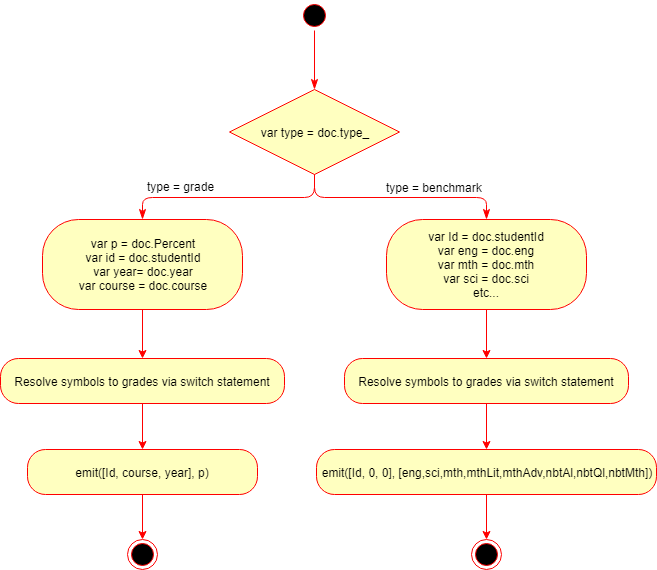
\includegraphics[scale=0.59]{./resources/figures/fig-mapfn-correlation-grades.png}
    \end{mdframed}
    \caption[\textit{Map}-function: \texorpdfstring{grades $\bowtie$ admissions}{Lg}]{\textbf{Figure \ref{fig-mapfn-correlation-grades}: \textit{Map}-function: \texorpdfstring{grades $\bowtie$ admissions}{Lg}}}
    \label{fig-mapfn-correlation-grades}
\end{figure}


\subsection{Presentation}
A list function is used for data retrieval; this function scans the index iteratively (i.e. documents for each student are processed iteratively; first a student's admissions document is processed, then a student's grades documents are processed). The 2-way join is achieved in this way; for every student number the grade and admissions data are joined, and summations of various fields of the grades and each benchmark are updated. For example, for every index key:value processed, the product of \mintinline{text}{CSC1015F \% x each benchmark \%} is calculated and added to running sums kept for each benchmark.

Once the iteration over student numbers is finished, the completed summations are used to calculate correlation coefficients for each combination of benchmarking method and grade  according to Equation \ref{eq:correlation}\footnote{\textit{x}: grade \%, \textit{y}: benchmark (\textit{r} is calculated for multiple \textit{y} values)}.

Although the \_stats reduce function calculates \textit{sum of squares} per dataset, this is not useful in cases where individual rows from separate entities should be joined (such as in this 2-way join). For example, the numerator (Equation \ref{eq:numerator}) from the correlation formula (Equation \ref{eq:correlation}) cannot be calculated during MapReduce. Only the $\sum{x}$ and $\sum{y}$ values are accessible when joining the two entities during list function executions, and not $x$ and $y$ values since these values come from entity instances.
\begin{align}
    N\sum{xy} - (\sum{x})(\sum{y})\label{eq:numerator}
\end{align}
Only aggregations of entity instances are available upon index retrieval (when retrieving reduced output) and not the individual instances. Similarly, the denominator of the formula also could not be calculated from the \_stats function output.

List function logic is represented as an activity diagram in Figure \ref{fig-listfn-correlation-grades} and is configured to output a table of correlation coefficients for each benchmarking method as shown in Table \ref{tbl-correlation-grades}.

\begin{figure}[H]
    \centering
    \begin{mdframed}
        \centering
        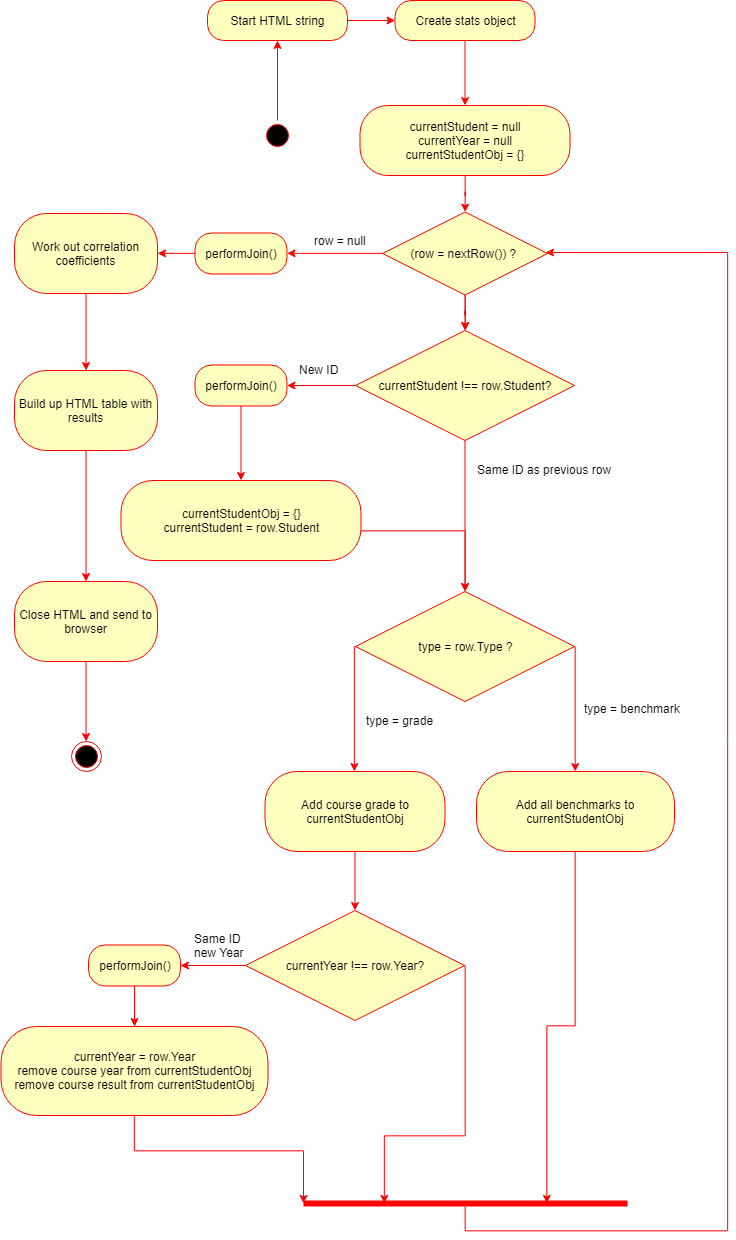
\includegraphics[scale=0.5]{./resources/figures/fig-listfn-correlation-grades.png}
    \end{mdframed}
    \caption[\textit{List}-function: \texorpdfstring{grades $\bowtie$ admissions}{Lg}]{\textbf{Figure \ref{fig-listfn-correlation-grades}: \textit{List}-function: \texorpdfstring{grades $\bowtie$ admissions}{Lg}}}
    \label{fig-listfn-correlation-grades}
\end{figure}
